\chapter{Object Design}
    \section{Legenda}
        Di seguito è riportato il diagramma di dettaglio delle classi nel dominio della soluzione del processo server e del processo client.\\
        In particolare, il tipo di visibilità è espressa da questa tabella:
        \begin{figure}[htbp!]
            \centering
            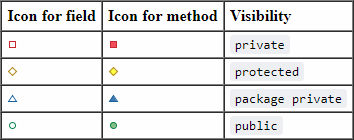
\includegraphics[width=0.25\linewidth]{Immagini/Legend visibility.png}
            \caption{Legenda della visibilità}
            \label{fig:Legenda della visibilità}
        \end{figure}\\
        Inoltre, i costruttori della classe sono i metodi contrassegnati da \textless{}\textless{}Create\textgreater{}\textgreater{}.

    \section{Class Diagram del dominio della soluzione del Server}
        %Class Diagram costruito con PlantUML
        \begin{figure}[htbp!]
            \centering
                \vspace{2\baselineskip}
                
\includegraphics[width=\linewidth]{Immagini/WorkInProgress.pdf}
            \caption{Class Diagram del dominio della soluzione del Server}
            \label{fig:Class Diagram del dominio della soluzione del Server}
        \end{figure}

    \section{Class Diagram del dominio della soluzione del Client}
        %Class Diagram costruito con PlantUML
        \begin{figure}[htbp!]
            \centering
                \vspace{2\baselineskip}
                
\includegraphics[width=\linewidth]{Immagini/WorkInProgress.pdf}
            \caption{Class Diagram del dominio della soluzione del Client}
            \label{fig:Class Diagram del dominio della soluzione del Client}
        \end{figure}